\documentclass[conference]{IEEEtran}
% Build: latexmk -pdf main.tex   (or: pdflatex main && bibtex main && pdflatex main && pdflatex main)
% Every number below comes from gen/*.tex, produced by make_assets.py from data/rigor/*.csv.
\usepackage{cite}
\usepackage{amsmath}
\usepackage{graphicx}
\usepackage{booktabs}
\usepackage{multirow}
\usepackage{xcolor}
\usepackage{listings}
\usepackage{tikz}
\usetikzlibrary{positioning,fit,arrows.meta}
\usepackage[hidelinks]{hyperref}
\usepackage{microtype}
\newcommand{\CpuClientMax}{0.022}
\newcommand{\CpuClientMin}{0.016}
\newcommand{\Excluded}{10}
\newcommand{\ExcludedNumerator}{10}
\newcommand{\Failures}{0}
\newcommand{\Hangs}{0}
\newcommand{\HtwoAFiftyTwo}{1.50}
\newcommand{\HtwoFFiftyTwo}{4.65}
\newcommand{\LossANgxFive}{5.01}
\newcommand{\LossANgxOne}{0.91}
\newcommand{\LossANgxTwo}{1.97}
\newcommand{\LossAQgoFive}{2.02}
\newcommand{\LossAQgoOne}{0.45}
\newcommand{\LossAQgoTwo}{0.57}
\newcommand{\LossATcpFive}{2.51}
\newcommand{\LossATcpOne}{0.34}
\newcommand{\LossATcpTwo}{0.94}
\newcommand{\LossBNgxFive}{4.68}
\newcommand{\LossBNgxOne}{0.96}
\newcommand{\LossBNgxTwo}{1.83}
\newcommand{\LossBQgoFive}{1.90}
\newcommand{\LossBQgoOne}{0.22}
\newcommand{\LossBQgoTwo}{0.72}
\newcommand{\LossBTcpFive}{3.03}
\newcommand{\LossBTcpOne}{0.41}
\newcommand{\LossBTcpTwo}{1.01}
\newcommand{\LossFNgxFive}{5.02}
\newcommand{\LossFNgxOne}{1.05}
\newcommand{\LossFNgxTwo}{2.05}
\newcommand{\LossFQgoFive}{4.89}
\newcommand{\LossFQgoOne}{1.05}
\newcommand{\LossFQgoTwo}{2.15}
\newcommand{\LossFTcpFive}{4.91}
\newcommand{\LossFTcpOne}{1.01}
\newcommand{\LossFTcpTwo}{2.20}
\newcommand{\NgxAFiftyTwo}{7.28}
\newcommand{\NgxFFiftyTwo}{7.38}
\newcommand{\PatchMaxSpeedup}{4.5}
\newcommand{\PatchMinSpeedup}{1.5}
\newcommand{\RatANgxFiftyFive}{2.50}
\newcommand{\RatANgxFiftyTwo}{4.69}
\newcommand{\RatANgxLossyMax}{6.11}
\newcommand{\RatANgxLossyMin}{1.88}
\newcommand{\RatANgxMax}{6.11}
\newcommand{\RatANgxMin}{1.23}
\newcommand{\RatAQgoLossyMax}{0.85}
\newcommand{\RatAQgoLossyMin}{0.52}
\newcommand{\RatAQgoMax}{0.85}
\newcommand{\RatAQgoMin}{0.52}
\newcommand{\RatFNgxFiftyFive}{1.08}
\newcommand{\RatFNgxFiftyTwo}{1.55}
\newcommand{\RatFNgxLossyMax}{2.10}
\newcommand{\RatFNgxLossyMin}{1.08}
\newcommand{\RatFNgxMax}{2.10}
\newcommand{\RatFNgxMin}{1.08}
\newcommand{\RatFNgxZeroHi}{36}
\newcommand{\RatFNgxZeroLo}{17}
\newcommand{\RatFQgoLossyMax}{0.88}
\newcommand{\RatFQgoLossyMin}{0.50}
\newcommand{\RatFQgoMax}{0.88}
\newcommand{\RatFQgoMin}{0.50}
\newcommand{\RatGNgxLossyMax}{2.72}
\newcommand{\RatGNgxLossyMin}{1.15}
\newcommand{\RatGNgxMax}{2.72}
\newcommand{\RatGNgxMin}{0.85}
\newcommand{\RatGNgxZeroHi}{15}
\newcommand{\RatGNgxZeroLo}{13}
\newcommand{\RatGQgoLossyMax}{0.77}
\newcommand{\RatGQgoLossyMin}{0.57}
\newcommand{\RatGQgoMax}{0.77}
\newcommand{\RatGQgoMin}{0.57}
\newcommand{\RatHNgxLossyMax}{2.62}
\newcommand{\RatHNgxLossyMin}{1.09}
\newcommand{\RatHNgxMax}{2.62}
\newcommand{\RatHNgxMin}{0.79}
\newcommand{\RatHQchLossyMax}{1.01}
\newcommand{\RatHQchLossyMin}{0.70}
\newcommand{\RatHQchMax}{1.01}
\newcommand{\RatHQchMin}{0.70}
\newcommand{\RatHQgoLossyMax}{0.94}
\newcommand{\RatHQgoLossyMin}{0.54}
\newcommand{\RatHQgoMax}{0.94}
\newcommand{\RatHQgoMin}{0.54}
\newcommand{\RatPNgxLossyMax}{1.31}
\newcommand{\RatPNgxLossyMin}{0.64}
\newcommand{\RatPNgxMax}{1.31}
\newcommand{\RatPNgxMin}{0.64}
\newcommand{\RatPQgoLossyMax}{0.81}
\newcommand{\RatPQgoLossyMin}{0.47}
\newcommand{\RatPQgoMax}{0.81}
\newcommand{\RatPQgoMin}{0.47}
\newcommand{\RcvbufAZero}{188}
\newcommand{\RcvbufFNgx}{7{,}673}
\newcommand{\RcvbufFQgo}{12}
\newcommand{\RcvbufG}{0}
\newcommand{\SigANgxFaster}{0}
\newcommand{\SigANgxLossyFaster}{0}
\newcommand{\SigANgxLossySlower}{6}
\newcommand{\SigANgxSlower}{8}
\newcommand{\SigAQgoFaster}{4}
\newcommand{\SigAQgoLossyFaster}{2}
\newcommand{\SigAQgoLossySlower}{0}
\newcommand{\SigAQgoSlower}{0}
\newcommand{\SigFNgxFaster}{0}
\newcommand{\SigFNgxLossyFaster}{0}
\newcommand{\SigFNgxLossySlower}{3}
\newcommand{\SigFNgxSlower}{5}
\newcommand{\SigFQgoFaster}{6}
\newcommand{\SigFQgoLossyFaster}{4}
\newcommand{\SigFQgoLossySlower}{0}
\newcommand{\SigFQgoSlower}{0}
\newcommand{\SigGNgxFaster}{2}
\newcommand{\SigGNgxLossyFaster}{0}
\newcommand{\SigGNgxLossySlower}{5}
\newcommand{\SigGNgxSlower}{5}
\newcommand{\SigGQgoFaster}{4}
\newcommand{\SigGQgoLossyFaster}{2}
\newcommand{\SigGQgoLossySlower}{0}
\newcommand{\SigGQgoSlower}{0}
\newcommand{\SigHNgxFaster}{2}
\newcommand{\SigHNgxLossyFaster}{0}
\newcommand{\SigHNgxLossySlower}{4}
\newcommand{\SigHNgxSlower}{4}
\newcommand{\SigHQchFaster}{3}
\newcommand{\SigHQchLossyFaster}{2}
\newcommand{\SigHQchLossySlower}{0}
\newcommand{\SigHQchSlower}{0}
\newcommand{\SigHQgoFaster}{5}
\newcommand{\SigHQgoLossyFaster}{3}
\newcommand{\SigHQgoLossySlower}{0}
\newcommand{\SigHQgoSlower}{0}
\newcommand{\SigPNgxFaster}{4}
\newcommand{\SigPNgxLossyFaster}{2}
\newcommand{\SigPNgxLossySlower}{0}
\newcommand{\SigPNgxSlower}{0}
\newcommand{\SigPQgoFaster}{7}
\newcommand{\SigPQgoLossyFaster}{5}
\newcommand{\SigPQgoLossySlower}{0}
\newcommand{\SigPQgoSlower}{0}
\newcommand{\TotalTransfers}{3,060}


\lstset{basicstyle=\ttfamily\scriptsize, columns=fullflexible, keepspaces=true, frame=b, framerule=0.4pt,
        numbers=none, xleftmargin=2pt, belowcaptionskip=4pt, escapeinside={(*@}{@*)}}
\newcommand{\hthree}{HTTP/3}
\newcommand{\htwo}{HTTP/2}

\begin{document}

\title{Equal Loss Is Not Equal: Emulator Placement, Receive Buffers,\\ and a One-Line Congestion-Control Bug Behind an
\hthree{} Loss Penalty}

% TODO(authors): confirm order and affiliations with both authors before submission.
% Affiliation and e-mail style follow Adith's other VIT manuscripts (AgentLint, ICMLDE 1717).
% TODO: add Abhilash's e-mail once confirmed (not guessed here).
\author{\IEEEauthorblockN{Abhilash Singh}
\IEEEauthorblockA{School of Computer Science and Engineering\\
Vellore Institute of Technology\\
Vellore, Tamil Nadu 632014, India}
\and
\IEEEauthorblockN{Adith Manikonda}
\IEEEauthorblockA{School of Computer Science and Engineering\\
Vellore Institute of Technology\\
Vellore, Tamil Nadu 632014, India\\
adith.manikonda2024@vitstudent.ac.in}}

\maketitle

\begin{abstract}
Testbed comparisons of \hthree{} over QUIC and \htwo{} over TCP disagree about which protocol suffers more from packet
loss. We started from a namespace-and-\texttt{netem} testbed in which nginx's \hthree{} was up to $\RatANgxLossyMax\times$
slower than \htwo{} under uniform random loss, and dissected that result with \TotalTransfers{} serial, instrumented
transfers across seven configurations. Three effects explain it. First, \texttt{netem} attached to a sender's own interface
drops whole segmentation-offload buffers, so at a nominal 2\,\% loss kernel TCP experienced only \LossATcpTwo\,\% loss
events per data packet, while nginx's QUIC, which sends one datagram per buffer, experienced \LossANgxTwo\,\%; disabling
offloads with \texttt{ethtool} does not fix this, but moving \texttt{netem} to a separate router namespace does. Equalising
loss shrinks the \hthree{} penalty at 50\,ms/2\,\% from $\RatANgxFiftyTwo\times$ to $\RatFNgxFiftyTwo\times$. Second,
client UDP receive-buffer overflow silently drops packets of unpaced QUIC senders and turns a 13--15\,\% \hthree{} advantage
at 0\,\% loss into a 17--36\,\% deficit. Third, the remaining penalty is specific to nginx: under equal loss quic-go and
Cloudflare quiche are never significantly slower than TCP, and qlog traces show nginx sustaining 4 packets per round
trip against quic-go's 11.5. We trace this to nginx's CUBIC computing the multiplicative decrease from bytes in flight
after the acknowledged and lost packets have been removed; changing that single line makes nginx
$\PatchMinSpeedup$--$\PatchMaxSpeedup\times$ faster under loss and removes every significant deficit to \htwo. We release the
testbed, data and analysis as a reproducible container, and give a checklist for QUIC-vs-TCP emulation studies.
\end{abstract}

\begin{IEEEkeywords}
QUIC, HTTP/3, network emulation, netem, congestion control, CUBIC, measurement methodology
\end{IEEEkeywords}

\section{Introduction}
QUIC~\cite{rfc9000} and \hthree~\cite{rfc9114} were designed in part to perform better than TCP and \htwo{} on lossy
paths: streams are independent, so a lost packet does not block unrelated data, and loss recovery~\cite{rfc9002} benefits
from unambiguous packet numbers. Measurement studies nevertheless disagree on how the two stacks compare under
loss~\cite{kakhki2017long,wolsing2019performance,yu2021dissecting,megyesi2016quick}, and several have observed that the
answer depends on the implementation and its configuration~\cite{yu2021dissecting,marx2020same,kakhki2017long}.

Many such comparisons, including course and lab projects, use the cheapest available testbed: two Linux network namespaces
joined by a virtual Ethernet (veth) pair, with \texttt{tc netem} configured on the endpoints' interfaces to add delay and
random loss. Our own testbed of this kind produced a clear result: at 2\,\% or more uniform loss, nginx's \hthree{} was
slower than \htwo{} in every tested cell, by up to several times. This paper asks whether that verdict describes the
protocols, the implementation, or the testbed.

The answer is all three, in a specific order. We make the following contributions:
\begin{itemize}
\item We show that \texttt{netem} on a sending endpoint applies the configured loss rate per kernel buffer rather than per
packet. Linux TCP always hands the qdisc multi-segment GSO buffers and quic-go batches datagrams with UDP GSO, so both see
roughly half the nominal loss events, while a sender without batching sees all of them (\S\ref{sec:placement}).
\texttt{ethtool} offload settings do not change this; a separate router namespace does.
\item We show that client UDP receive-buffer overflow is a second, host-dependent source of loss that affects only
unpaced QUIC senders and reverses the 0\,\%-loss verdict (\S\ref{sec:rcvbuf}).
\item Under equal per-packet loss, two mature QUIC stacks (quic-go, quiche) match or beat kernel TCP in every cell, while
nginx remains up to $\RatGNgxLossyMax\times$ slower (\S\ref{sec:impl}).
\item Using qlog and a one-line intervention, we trace nginx's deficit to the way its CUBIC multiplicative decrease reads
bytes in flight, and quantify the effect of changing it (\S\ref{sec:rootcause}).
\item We publish the full testbed as a pinned container, all \TotalTransfers{} transfer records with per-transfer kernel
counters, and the scripts that generate every number in this paper.
\end{itemize}

\section{Background}\label{sec:background}
\textbf{netem and segmentation offload.} \texttt{netem} is a queueing discipline: it decides whether to drop a packet when
the kernel enqueues a socket buffer (skb) on the device~\cite{linuxnetem}. With generic segmentation offload
(GSO)~\cite{linuxgso}, the TCP stack builds skbs that carry many MSS-sized segments and splits them only after the qdisc,
or in the NIC. Linux TCP always uses GSO internally, whatever the device advertises. On the UDP side, QUIC stacks such
as quic-go use UDP GSO (\texttt{UDP\_SEGMENT}) to pass several datagrams to the kernel in one call. One \texttt{netem}
``loss'' on such an skb removes a burst of packets that the sender then detects as a single loss event. \texttt{netem}'s
loss accuracy has been studied in isolation~\cite{jurgelionis2011netem}; its interaction with sender-side batching has, to our
knowledge, only been discussed informally.

\textbf{Receive buffers.} On fast emulated links, a user-space QUIC receiver may not drain its UDP socket fast enough;
datagrams that do not fit into the socket buffer are counted in \texttt{Udp RcvbufErrors} and dropped before QUIC sees
them. Zhang et al.\ showed that receiver-side processing limits QUIC on fast links~\cite{zhang2024quic}; Jaeger et
al.\ examined buffer sizes and offloads for QUIC throughput~\cite{jaeger2023highway,kempf2024fastlane}.

\textbf{CUBIC multiplicative decrease.} On a congestion event CUBIC sets
$\mathit{ssthresh} = \beta \cdot \mathit{flight\_size}$ with $\beta = 0.7$, where flight size is the amount of
outstanding data~\cite{rfc9438,rfc5681}. RFC~9438 permits implementations to use the congestion window instead, provided they
prevent the window from growing while the sender is application-limited. RFC~9002's reference pseudocode for QUIC reduces
from the congestion window~\cite{rfc9002}.

\section{Testbed and Method}\label{sec:method}

\begin{figure}[t]
\centering
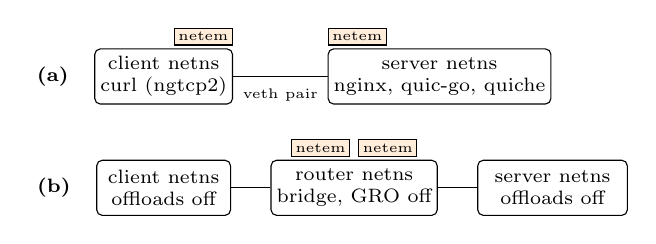
\begin{tikzpicture}[font=\scriptsize, node distance=4mm,
  ns/.style={draw, rounded corners=2pt, minimum height=7mm, align=center, inner sep=2pt},
  em/.style={draw, fill=orange!15, inner sep=1.5pt, font=\tiny}]
\node[ns, minimum width=17mm] (c1) {client netns\\ curl (ngtcp2)};
\node[ns, minimum width=19mm, right=12mm of c1] (s1) {server netns\\ nginx, quic-go, quiche};
\draw[-] (c1) -- node[below=1pt, font=\tiny]{veth pair} (s1);
\node[em, anchor=south west] at ([yshift=1pt]s1.north west) {netem};
\node[em, anchor=south east] at ([yshift=1pt]c1.north east) {netem};
\node[anchor=east, font=\scriptsize\bfseries] at ([xshift=-2mm]c1.west) {(a)};
\node[ns, minimum width=17mm, below=7mm of c1] (c2) {client netns\\ offloads off};
\node[ns, minimum width=15mm, right=5mm of c2] (r2) {router netns\\ bridge, GRO off};
\node[ns, minimum width=19mm, right=5mm of r2] (s2) {server netns\\ offloads off};
\draw (c2) -- (r2) -- (s2);
\node[em, anchor=south west] at ([yshift=1pt,xshift=0.5mm]r2.north) {netem};
\node[em, anchor=south east] at ([yshift=1pt,xshift=-0.5mm]r2.north) {netem};
\node[anchor=east, font=\scriptsize\bfseries] at ([xshift=-2mm]c2.west) {(b)};
\end{tikzpicture}
\caption{Topologies. (a) \texttt{netem} on the endpoints' own veth devices (configurations A, B; the original testbed).
(b) \texttt{netem} on the egress ports of a separate router namespace, so it sees wire-sized packets (F, G, D, P, H).
Each \texttt{netem} adds half the RTT, the loss rate and a 1\,Gbit/s rate in one direction.}
\label{fig:topo}
\end{figure}

\textbf{Testbed.} Fig.~\ref{fig:topo} shows the two topologies. All software runs in one privileged Docker container
(Ubuntu 22.04) on Docker Desktop's Linux 6.10 VM (8 vCPUs, 8\,GB) on an Apple M3 host. The client is curl 8.23.1-DEV built
with ngtcp2, nghttp3 and OpenSSL 3.6.5~\cite{ngtcp2}. Four senders serve the same 1\,MB object over TLS: nginx 1.31.9
over \htwo{} (kernel TCP, CUBIC) and over \hthree{} using its native QUIC module~\cite{nginx}, a quic-go v0.64.1
\hthree{} file server~\cite{quicgo}, and Cloudflare quiche 0.29.3's \texttt{quiche-server}~\cite{quiche}. All QUIC senders
use CUBIC. Every source is pinned to an exact commit and built in a Dockerfile.

\textbf{Procedure.} Each transfer is a fresh curl process and connection, so completion time includes the handshake.
Transfers run strictly one at a time. The client and each server are pinned to separate vCPUs, and the order of senders is
rotated every iteration to cancel drift. The grid is RTT $\in\{50, 100\}$\,ms $\times$ uniform loss
$\in\{0,1,2,5\}$\,\% applied in both directions, with 20 iterations per sender and cell and a 40\,s cap (no transfer hit
it). Before measuring, each sender must serve the object over the intended HTTP version on a clean link. For every
transfer we record curl's timings, client and server CPU time, and kernel counters: \texttt{netem} sent and dropped
packets in each direction, TCP \texttt{RetransSegs}, and client \texttt{Udp RcvbufErrors}. The realised loss rate is
therefore measured rather than assumed.

\textbf{Statistics.} Because absolute times drift between runs, the primary metric is the median of per-iteration paired
ratios (\hthree{} time / \htwo{} time in the same iteration), with a 2000-sample bootstrap 95\,\% CI. A difference is called
significant when the CI excludes 1 and a Wilcoxon signed-rank test is significant at 0.05 after Bonferroni correction over
all comparisons in that configuration (16, or 24 for H).

\textbf{Data hygiene.} The host idled to sleep three times during unattended runs, suspending the VM. We drop any transfer
whose wall-clock gap to the previous transfer exceeds its own duration by more than 60\,s (\Excluded{} transfers in total);
later runs prevented sleep. The process-hang guard never fired, and there were \Failures{} failed transfers.

\begin{table}[t]
\centering
\caption{Configurations. $n$ = transfers after exclusions.}
\label{tab:configs}
\footnotesize
\begin{tabular}{@{}clcclr@{}}
\toprule
Cfg & netem on & Offl. & rcvbuf & HTTP senders & $n$ \\
\midrule
A & endpoint veth & on & 208\,KB & h2, nginx, quic-go & 479 \\
B & endpoint veth & off & 208\,KB & h2, nginx, quic-go & 480 \\
F & router netns & off & 208\,KB & h2, nginx, quic-go & 480 \\
G & router netns & off & 4\,MB & h2, nginx, quic-go & 480 \\
D & router netns & off & 4\,MB & nginx, quic-go + qlog & 30 \\
P & router netns & off & 4\,MB & h2, \emph{patched} nginx, quic-go & 477 \\
H & router netns & off & 4\,MB & h2, nginx, quic-go, quiche & 634 \\
\bottomrule
\end{tabular}

\end{table}

Table~\ref{tab:configs} lists the configurations. A reproduces the original testbed settings. B turns endpoint offloads off
with \texttt{ethtool}. F moves \texttt{netem} to the router. G additionally raises the client's default UDP receive buffer
from 208\,KB to 4\,MB. D repeats one cell of G with qlog~\cite{qlog} enabled. P is G with a one-line change to nginx
(\S\ref{sec:rootcause}). H is G with all four senders in the same run.

\section{Pitfall 1: Where netem Sits}\label{sec:placement}

\begin{figure}[t]
\centering
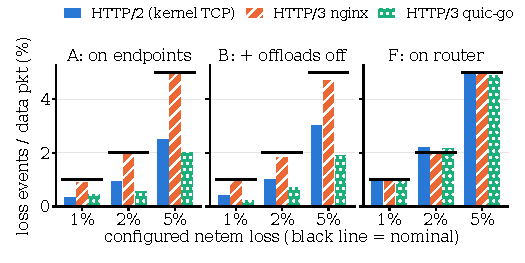
\includegraphics[width=\columnwidth]{figs/fig_loss.pdf}
\caption{Realised loss events per data packet (\texttt{netem} drops on the data path / packets offered), median over 20
transfers per bar, 50\,ms RTT. On an endpoint (A, B) TCP and quic-go see about half the configured loss; on a router (F)
all senders see it.}
\label{fig:loss}
\end{figure}

Fig.~\ref{fig:loss} shows the loss each sender actually experienced. With \texttt{netem} on the endpoint (A), a nominal
2\,\% produced \LossATcpTwo\,\% loss events per data packet for TCP, \LossAQgoTwo\,\% for quic-go and \LossANgxTwo\,\% for
nginx's QUIC; at 5\,\% the figures are \LossATcpFive, \LossAQgoFive{} and \LossANgxFive\,\%. nginx sends one datagram per
system call, so each of its packets is its own skb. TCP and quic-go hand the qdisc multi-packet buffers, and one drop
decision removes the whole buffer. To the sender, a burst of consecutive losses within one round trip costs about as
much as a single loss: both TCP and QUIC reduce their window once per round trip. So in the original testbed, nginx's
QUIC was in effect tested at roughly twice the loss rate of TCP.

Turning off TSO, GSO and GRO on the endpoint veths (B) barely changes this (TCP \LossBTcpTwo\,\%, quic-go \LossBQgoTwo\,\%,
nginx \LossBNgxTwo\,\% at 2\,\%). The device features only control whether segmentation happens in the device. The TCP
stack and \texttt{UDP\_SEGMENT} still build multi-packet skbs above the qdisc, and software segmentation then happens
after \texttt{netem} has decided. Only moving \texttt{netem} off the senders equalises loss. In F, packets are segmented
before they leave the sender namespace, the router does not re-aggregate them, and all three senders see
\LossFTcpTwo, \LossFNgxTwo{} and \LossFQgoTwo\,\% at a nominal 2\,\%.

\textbf{Effect on the verdict.} Table~\ref{tab:ratios} compares A and F. nginx's own completion time is unchanged
(\NgxAFiftyTwo\,s in A vs.\ \NgxFFiftyTwo\,s in F at 50\,ms/2\,\%), while \htwo{} becomes much slower (\HtwoAFiftyTwo\,s to
\HtwoFFiftyTwo\,s) once it receives the full loss. The \hthree/\htwo{} ratio falls from $\RatANgxFiftyTwo$ to
$\RatFNgxFiftyTwo$ at 2\,\% and from $\RatANgxFiftyFive$ to $\RatFNgxFiftyFive$ (not significant) at 5\,\%. Most of the
reported \hthree{} loss penalty was TCP being tested at a lower loss rate.

\begin{table*}[t]
\centering
\caption{Median paired completion-time ratio \hthree{} / \htwo{} per cell and configuration (\,$<1$: \hthree{} faster).
\textbf{Bold}$^{\uparrow}$/\textbf{bold}$^{\downarrow}$: significantly slower/faster (bootstrap CI excludes 1 and
Bonferroni-corrected Wilcoxon $p<0.05$). Second column: \htwo{} median time in G for scale.
$^\dagger$P uses the patched nginx (\S\ref{sec:rootcause}).}
\label{tab:ratios}
\footnotesize
\begin{tabular}{@{}lr|rrrr|r|rrrr|r@{}}
\toprule
 & HTTP/2 & \multicolumn{5}{c|}{nginx HTTP/3 / HTTP/2} & \multicolumn{4}{c|}{quic-go / HTTP/2} & quiche \\
RTT, loss & G (s) & A & F & G & H & P$^\dagger$ & A & F & G & H & H \\
\midrule
50\,ms, 0\,\% & 0.55 & \textbf{1.23}$^{\uparrow}$ & \textbf{1.17}$^{\uparrow}$ & \textbf{0.85}$^{\downarrow}$ & \textbf{0.79}$^{\downarrow}$ & \textbf{0.81}$^{\downarrow}$ & \textbf{0.62}$^{\downarrow}$ & \textbf{0.61}$^{\downarrow}$ & \textbf{0.63}$^{\downarrow}$ & \textbf{0.60}$^{\downarrow}$ & \textbf{0.84}$^{\downarrow}$ \\
50\,ms, 1\,\% & 1.62 & \textbf{3.54}$^{\uparrow}$ & 2.10 & \textbf{2.72}$^{\uparrow}$ & \textbf{1.86}$^{\uparrow}$ & 1.31 & 0.65 & 0.88 & 0.70 & 0.61 & 0.97 \\
50\,ms, 2\,\% & 4.29 & \textbf{4.69}$^{\uparrow}$ & \textbf{1.55}$^{\uparrow}$ & \textbf{1.63}$^{\uparrow}$ & \textbf{1.49}$^{\uparrow}$ & 0.84 & 0.76 & \textbf{0.61}$^{\downarrow}$ & 0.62 & \textbf{0.62}$^{\downarrow}$ & 0.84 \\
50\,ms, 5\,\% & 9.58 & \textbf{2.50}$^{\uparrow}$ & 1.08 & \textbf{1.15}$^{\uparrow}$ & 1.22 & \textbf{0.64}$^{\downarrow}$ & \textbf{0.52}$^{\downarrow}$ & \textbf{0.50}$^{\downarrow}$ & \textbf{0.57}$^{\downarrow}$ & \textbf{0.58}$^{\downarrow}$ & \textbf{0.78}$^{\downarrow}$ \\
\midrule
100\,ms, 0\,\% & 0.99 & \textbf{1.34}$^{\uparrow}$ & \textbf{1.36}$^{\uparrow}$ & \textbf{0.87}$^{\downarrow}$ & \textbf{0.89}$^{\downarrow}$ & \textbf{0.87}$^{\downarrow}$ & \textbf{0.68}$^{\downarrow}$ & \textbf{0.70}$^{\downarrow}$ & \textbf{0.69}$^{\downarrow}$ & \textbf{0.70}$^{\downarrow}$ & 0.89 \\
100\,ms, 1\,\% & 4.44 & \textbf{4.23}$^{\uparrow}$ & \textbf{1.99}$^{\uparrow}$ & \textbf{2.07}$^{\uparrow}$ & \textbf{2.62}$^{\uparrow}$ & 0.66 & 0.85 & 0.76 & 0.77 & 0.94 & 1.01 \\
100\,ms, 2\,\% & 7.72 & \textbf{6.11}$^{\uparrow}$ & \textbf{2.02}$^{\uparrow}$ & \textbf{1.60}$^{\uparrow}$ & \textbf{1.51}$^{\uparrow}$ & \textbf{0.65}$^{\downarrow}$ & 0.78 & \textbf{0.50}$^{\downarrow}$ & 0.64 & 0.79 & 0.85 \\
100\,ms, 5\,\% & 17.04 & \textbf{1.88}$^{\uparrow}$ & 1.10 & 1.23 & 1.09 & 0.87 & \textbf{0.56}$^{\downarrow}$ & \textbf{0.59}$^{\downarrow}$ & \textbf{0.59}$^{\downarrow}$ & \textbf{0.54}$^{\downarrow}$ & \textbf{0.70}$^{\downarrow}$ \\
\bottomrule
\end{tabular}

\end{table*}

\begin{figure*}[t]
\centering
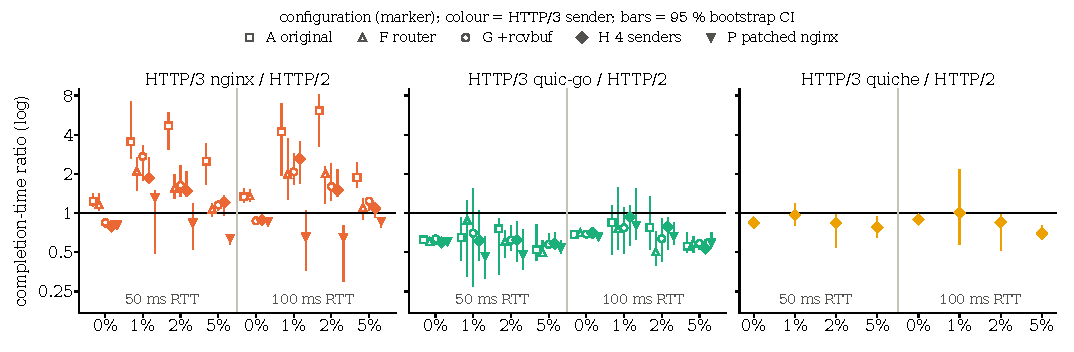
\includegraphics[width=\textwidth]{figs/fig_ratio.pdf}
\caption{Paired \hthree/\htwo{} completion-time ratios with 95\,\% bootstrap CIs per sender (panel), cell (x) and
configuration (marker). Moving \texttt{netem} to a router (A$\to$F) collapses most of nginx's penalty. quic-go and quiche
stay at or below 1 throughout. Patching nginx (P) moves it below 1 under loss.}
\label{fig:ratio}
\end{figure*}

\section{Pitfall 2: The Receiver's UDP Buffer}\label{sec:rcvbuf}
At 0\,\% configured loss, nginx's \hthree{} transfers in A lost a median of \RcvbufAZero{} datagrams each to client
receive-buffer overflow, while TCP and quic-go lost none. In F, nginx accumulated \RcvbufFNgx{} \texttt{RcvbufErrors} over its
transfers against \RcvbufFQgo{} for quic-go. nginx bursts a full window without pacing into a 208\,KB default buffer, while
quic-go paces its sending. These drops are invisible to \texttt{netem}'s counters and act as extra, sender-specific loss.

With a 4\,MB buffer (G, H, P) we observed \RcvbufG{} receive-buffer errors, and the 0\,\%-loss verdict reverses: nginx
\hthree{} becomes \RatGNgxZeroLo--\RatGNgxZeroHi\,\% \emph{faster} than \htwo{}, consistent with QUIC's one-round-trip
handshake saving~\cite{langley2017quic}, where in F it was \RatFNgxZeroLo--\RatFNgxZeroHi\,\% slower. The default buffer
size differs between distributions and virtualisation layers, so this verdict can change between hosts without any change to
the protocols. Median client CPU time per 1\,MB transfer was \CpuClientMin--\CpuClientMax\,s for all senders, so with serial
transfers CPU was not the bottleneck.

\section{Under Equal Loss, the Implementation Decides}\label{sec:impl}
With loss equalised and receive buffers fixed, Table~\ref{tab:ratios} (columns G and H) and Fig.~\ref{fig:ratio} separate
the senders cleanly. In H, where all four senders share one run:
\begin{itemize}
\item quic-go is never significantly slower than \htwo{} (ratios \RatHQgoMin--\RatHQgoMax) and is significantly faster
in \SigHQgoFaster{} of 8 cells;
\item quiche is never significantly slower (\RatHQchMin--\RatHQchMax) and is significantly faster in \SigHQchFaster{} of 8;
\item stock nginx is significantly slower in \SigHNgxLossySlower{} of 6 lossy cells (up to $\RatHNgxLossyMax\times$), and
faster only at 0\,\% loss.
\end{itemize}
Fig.~\ref{fig:cdf}(a) shows the full distributions at 50\,ms/2\,\%. The two mature QUIC stacks complete faster than TCP
across the whole distribution, and nginx is slower across the whole distribution. nginx's pattern in H matches G, which
ran hours earlier, so it is not run-to-run drift. The \hthree{} loss penalty seen in the original testbed is therefore a
property of one QUIC sender, made larger by two testbed artefacts. It is not a property of the protocol.

\begin{figure}[t]
\centering
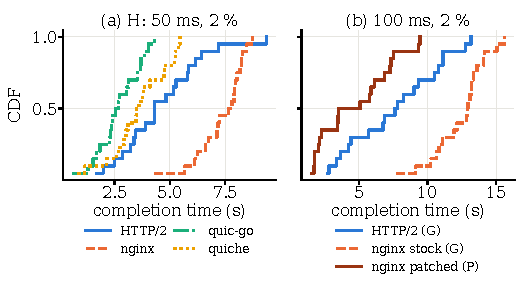
\includegraphics[width=\columnwidth]{figs/fig_cdf.pdf}
\caption{Completion-time CDFs, 20 transfers per line. (a) All four senders in one run (H) at 50\,ms RTT, 2\,\% loss.
(b) Stock nginx (G), patched nginx (P) and \htwo{} (G) at 100\,ms, 2\,\%.}
\label{fig:cdf}
\end{figure}

\section{Root Cause in nginx's CUBIC}\label{sec:rootcause}
\textbf{Symptom.} Run D repeats 50\,ms/2\,\% with qlog enabled at the client and on the quic-go server (nginx does not
emit qlog). Neither QUIC sender shows long idle periods driven by probe timeouts. What differs is the steady sending rate.
The client receives a median of 4.0 packets per 50\,ms round trip from nginx and 11.5 from quic-go, whose congestion
window has a time-weighted median of 13.9 packets. An AIMD sender at $p=0.02$ is expected to sustain about
$1.22/\sqrt{p}\approx 8.6$ packets per round trip~\cite{mathis1997macroscopic}. nginx sends at less than half of that, so its
window is held below what its own CUBIC should reach.

\textbf{Cause.} Listing~\ref{lst:nginx} shows nginx's congestion-event handler. It runs from loss detection, which nginx
performs at the end of processing an ACK frame. By then the bytes of every newly acknowledged packet have been subtracted
from \texttt{in\_flight}, and the handler subtracts the lost packet's bytes before computing the new threshold. When an
ACK both acknowledges a run of packets and declares one lost, which is the common case under random loss,
\texttt{in\_flight} at that point can be well below both the window and the amount outstanding at the moment of the loss.
The decrease then becomes much deeper than $\beta$, and it repeats at every congestion event.

\begin{lstlisting}[caption={Congestion-event handler in nginx's QUIC module (abridged)},
  label={lst:nginx}, float=t]
blocked = (cg->in_flight >= cg->window) ? 1 : 0;
cg->in_flight -= f->plen;       /* lost packet removed */
...
/* RFC 9438, 4.6. Multiplicative Decrease */
cg->recovery_start = now;
cg->w_prior = cg->window;
cg->w_max = (cg->window < cg->w_max)
          ? cg->window * (10 + NGX_QUIC_CUBIC_BETA) / 20
          : cg->window;
/* P changes in_flight to window in the next line */
cg->ssthresh = cg->in_flight * NGX_QUIC_CUBIC_BETA / 10;
cg->window = ngx_max(cg->ssthresh, cg->mtu * 2);
\end{lstlisting}

\textbf{Intervention.} We rebuilt the same nginx commit with only the marked line changed to reduce from
\texttt{cg->window}, which is the reduction in RFC~9002's reference pseudocode, and repeated G (configuration P).
Table~\ref{tab:patch} shows the result. Loss-free performance is unchanged, because the change touches only the
congestion-event path. Under loss, nginx becomes $\PatchMinSpeedup$--$\PatchMaxSpeedup\times$ faster. Its ratio to
\htwo{} drops to \RatPNgxLossyMin--\RatPNgxLossyMax{} (Table~\ref{tab:ratios}, column P). It is significantly slower than
\htwo{} in \SigPNgxLossySlower{} of 6 lossy cells, compared with \SigGNgxLossySlower{} for stock nginx in G, and
significantly faster in \SigPNgxLossyFaster. Fig.~\ref{fig:cdf}(b) shows the shift at 100\,ms/2\,\%.

\begin{table}[t]
\centering
\caption{Median nginx \hthree{} completion time, stock (G) vs.\ one-line patch (P).}
\label{tab:patch}
\footnotesize
\begin{tabular}{@{}lrrr@{}}
\toprule
RTT, loss & stock (G), s & patched (P), s & speed-up \\
\midrule
50\,ms, 0\,\% & 0.47 & 0.47 & 1.00$\times$ \\
50\,ms, 1\,\% & 4.58 & 2.05 & 2.24$\times$ \\
50\,ms, 2\,\% & 6.86 & 3.77 & 1.82$\times$ \\
50\,ms, 5\,\% & 11.19 & 6.73 & 1.66$\times$ \\
100\,ms, 0\,\% & 0.87 & 0.88 & 0.99$\times$ \\
100\,ms, 1\,\% & 8.14 & 1.81 & 4.49$\times$ \\
100\,ms, 2\,\% & 12.95 & 4.31 & 3.00$\times$ \\
100\,ms, 5\,\% & 20.40 & 13.73 & 1.49$\times$ \\
\bottomrule
\end{tabular}

\end{table}

\textbf{Interpretation.} Reducing from bytes in flight is permitted by RFC~9438~\cite{rfc9438}; the defect is
\emph{when} nginx samples it. Our change shows that this one line explains most of nginx's deficit. We do not propose it
as the upstream fix: a sender that reduces from the window must also prevent window growth while application-limited, and
we have not audited nginx's growth path for that. A conservative fix would record the flight size before the ACK frame is
processed and use that value in the decrease. We plan to report the issue to the nginx maintainers with this data.

\section{Related Work}\label{sec:related}
Early QUIC-vs-TCP comparisons found QUIC ahead on lossy and high-delay paths, with large variation across configurations
and versions~\cite{langley2017quic,megyesi2016quick,biswal2016quic,kakhki2017long}. Kakhki et al.~\cite{kakhki2017long}
stressed calibrated, instrumented comparisons. Wolsing et al.~\cite{wolsing2019performance} argued that fair comparisons
need equally tuned stacks. Yu and Benson~\cite{yu2021dissecting} showed that production QUIC performance depends heavily on
implementation and congestion-control choices. Marx et al.~\cite{marx2020same} documented wide behavioural diversity
across 15 QUIC implementations and introduced qlog-based root-cause analysis, which we use. Jaeger et al.\ and Kempf et
al.~\cite{jaeger2023highway,kempf2024fastlane} studied buffer sizes and offloads for QUIC throughput on high-rate links,
and Zhang et al.~\cite{zhang2024quic} identified receiver-side limits. Endres et al.~\cite{endres2022satellite} found large
differences between QUIC stacks under loss on satellite paths. Our work differs in focus: we quantify how emulator
placement biases the \emph{loss} each protocol experiences, show that \texttt{ethtool} does not remove the bias, and carry
one implementation's residual penalty down to a single line of code with an intervention.

\section{Recommendations}\label{sec:recs}
For QUIC-vs-TCP comparisons on Linux emulation testbeds:
\begin{enumerate}
\item Do not attach \texttt{netem} to a sender's own interface. Use a separate forwarding namespace or host with GRO off,
and segment on the endpoints.
\item Measure realised loss per sender from \texttt{netem}'s counters, or a capture, rather than reporting the configured rate.
\item Log \texttt{Udp RcvbufErrors} and size the client's socket buffer explicitly; report it.
\item Compare more than one QUIC implementation before attributing a result to the protocol, and record each one's
congestion controller and pacing.
\item Run transfers serially, pin processes, rotate sender order, and use within-iteration paired comparisons.
\item Check host power management and wall-clock gaps on laptops and VMs.
\end{enumerate}

\section{Limitations}\label{sec:limits}
All runs used one host type, Docker Desktop's Linux VM on Apple silicon. The placement effect follows from kernel
mechanisms that are not specific to it, but we have not yet repeated A vs.\ F on bare metal or on the original WSL2 host. We
test one object size (1\,MB), uniform random loss, two RTTs, an unconstrained 1\,Gbit/s rate (no bottleneck queue), CUBIC
everywhere, and a single client implementation, so ACK-frequency and flow-control effects on the client side are not
varied. Configurations ran sequentially over about a day, so comparisons of absolute times across configurations include
drift; our conclusions rest on within-run paired ratios, and on H, which compares all senders in one run. We infer nginx's
sending rate from client-side qlog because nginx does not export qlog.

\section{Conclusion}
A simple namespace testbed reported that \hthree{} suffers badly under packet loss. Most of that result came from where
\texttt{netem} was attached and from the client's receive buffer. The rest came from one line in one implementation's
congestion controller. With equal loss, two mature QUIC stacks match or beat kernel TCP, and nginx does too once that line
is changed. Testbed papers comparing transports should measure the loss they actually apply, and should not attribute a
single implementation's behaviour to the protocol.

\section*{Artifact Availability}
The container definitions, harness, raw per-transfer CSVs, qlog traces and the script that generates every number, table
and figure in this paper are available at \url{https://github.com/abhi-s99/quic-testbed} (branch \texttt{rigor/clean-rerun}).
% TODO: confirm the public URL/branch once pushed.

\bibliographystyle{IEEEtran}
\bibliography{refs}

\end{document}
